\documentclass{beamer}

\usepackage{amsfonts}
\usepackage{amsmath}
\usepackage{longtable}
\usepackage{csquotes}
\usepackage{standalone}

\usepackage{graphicx}
\graphicspath{{../pictures/}}

\usepackage{tikz}
\usetikzlibrary{shapes, calc, arrows, decorations.markings,
  decorations.pathmorphing, decorations, patterns, chains, snakes,
  backgrounds, positioning, fit, petri}
\newcommand{\inputpicture}[1]{\input{../drawings/#1}}

\usepackage{listings}
\lstset{language=C, basicstyle=\ttfamily, breaklines=true, keepspaces=true,
  keywordstyle=\color{blue}}

\usepackage{bytefield}

\usefonttheme{professionalfonts}
\usefonttheme{serif}
\usepackage{fontspec}
\setromanfont{CMU Serif}
\setsansfont{CMU Sans Serif}
\setmonofont{CMU Typewriter Text}

\usepackage{hyperref}
\hypersetup{colorlinks=true, linkcolor=black, filecolor=black, citecolor=black,
  urlcolor=blue , pdfauthor=Evgenii Iuliugin <yulyugin@gmail.com>,
  pdftitle=Fundamentals of Full-Platform Simulation}

\usepackage{underscore}
\usepackage{amsthm}

\subtitle{Fundamentals of Full-Platform Simulation}
\subject{Lecture}
\date{\today}

\author[Evgenii Iuliugin]{
  Evgenii Iuliugin, \small{\href{mailto:yulyugin@gmail.com}{yulyugin@gmail.com}}}
\typeout{Copyright 2021 Evgenii Iuliugin}

\usetheme{Madrid}
\setbeamertemplate{navigation symbols}{}

\makeatletter
\setbeamertemplate{footline}{%
  \leavevmode%
  \hbox{%
    \begin{beamercolorbox}[wd=.15\paperwidth,ht=2.25ex,dp=1ex,center]{author in head/foot}%
      \usebeamerfont{author in head/foot}\insertshortauthor\expandafter\ifblank\expandafter{\beamer@shortinstitute}{}{~~(\insertshortinstitute)}
    \end{beamercolorbox}%
    \begin{beamercolorbox}[wd=.77\paperwidth,ht=2.25ex,dp=1ex,center]{title in head/foot}%
      \usebeamerfont{title in head/foot}\insertshorttitle
    \end{beamercolorbox}%
  }%
  \begin{beamercolorbox}[wd=.08\paperwidth,ht=2.25ex,dp=1ex,right]{date in head/foot}%
    \usebeamerfont{date in head/foot}%
    \usebeamertemplate{page number in head/foot}%
    \hspace*{2ex}
  \end{beamercolorbox}
  \vskip0pt%
}
\makeatother

\newcommand{\startslides}{
  {\setbeamertemplate{footline}{}
  \begin{frame}
      \maketitle
  \end{frame}
  }

  \addtocounter{framenumber}{-1}

  \begin{frame}{\inserttitle}
      \tableofcontents
  \end{frame}
}

\newcommand{\finalslide}{{
  \setbeamertemplate{footline}{}

  \begin{frame}

  {\huge{Thank you!}\par}

  \vfill
  Slides and material are available at
  \url{https://github.com/yulyugin/sim-lectures}
  \vfill

  \tiny{\textit{Note}: All trademarks are the property of their respective
    owners. The presented point of view reflects the personal opinion of
    the author.

    %All the materials are licensed under the Creative Commons
    %Attribution-NonCommercial-ShareAlike 4.0 Worldwide. To view a copy of this
    %license, visit \url{http://creativecommons.org/licenses/by-nc-sa/4.0/}.
  }
  \end{frame}
}\addtocounter{framenumber}{-1}}

\title{Simulation Through Direct Execution}

\begin{document}

\startslides

\begin{frame}{On the Previous Lectures:}
Processor simulation:
\begin{itemize}
\item Interpreters (switched, threaded, cached) --- \textbf{slow}.
\item Binary translators (templates, IR) --- \textbf{faster} but still
  \textbf{slow}.
\end{itemize}
\end{frame}

\begin{frame}{Questions}
\begin{itemize}
\item What is the difference between compilation and translation?\pause
\item Is binary translation always faster than interpretation?\pause~No.
  When binary translation is slower than interpretation?\pause
\item Is static binary translation always possible?\pause~No. Why?\pause
\item What pipeline stages are optimized by a binary translator?
\end{itemize}
\end{frame}

\begin{frame}{Simulated System}
\centering
\vfill
\inputpicture{cpu-mem}
\vfill
\end{frame}

\section{Direct Execution}

\begin{frame}{When Direct Execution Is Possible?}
Idea: No simulation at all!

\bigskip
Direct Execution:
\begin{itemize}
\item If guest ISA is the same as host ISA.
\item Well... Or almost the same.
\end{itemize}
\end{frame}

\begin{frame}[fragile]{Algorithm}
\begin{verbatim}
execute() {
    save_host_ctx();
    set_guest_ctx();
    setjmp(back);
    goto guest_start_ip;
    back: restore_host_ctx();
}
\end{verbatim}
\end{frame}

\begin{frame}{Why Won't This Work?}
\pause
\begin{itemize}
\item Guest and host ISAs may not be exactly the same.
\item Different position of external resources (devices and memory).
\item Privileged instructions.
\item Isolation requirement.
\end{itemize}
\end{frame}

\begin{frame}{Why Won't This Work?}
\texttt{add \%r1, \%r2} \hfill OK

\texttt{mul \$10, \%r3}

\texttt{sub \%r11, \%r1}

\texttt{mov \$16, \%r13}

\medskip

\texttt{\textcolor{red}{div} \%r4, \%r5} \hfill Not supported by host

\medskip

\texttt{ld (\textcolor{red}{0xa000}), \%r10} \hfill Guest memory is at different address

\texttt{st \%r10, (\%r11)}

\medskip

\texttt{mov \%r13, \textcolor{red}{\%cr0}} \hfill Privileged instruction

\texttt{\textcolor{red}{trap} \$32}
\end{frame}

\section{Preliminary Scanning}

\begin{frame}{Preliminary Code Scanning}
\begin{itemize}
\item Inspect guest code for <<dangerous>> instructions before execution.
\item Replace (part of) the instructions by controlled --- \textit{instrumentation}.
\pause
\item{<<Almost>> binary translation.}
\end{itemize}
\end{frame}

\begin{frame}{Stubs and Patches}
\begin{tabular}{llr}
Source Code                     &    After Instrumentation               \\
\texttt{add \%r1, \%r2}         &    \texttt{add \%r1, \%r2}             \\
\texttt{mul \$10, \%r3}         &    \texttt{mul \$10, \%r3}             \\
\texttt{div \%r4, \%r5}         &    \texttt{trap \$255}         & stub  \\
\texttt{ld (0xa000), \%r10}     &    \texttt{ld (0xb000), \%r10} & patch \\
\texttt{st \%r10, (\%r11)}      &    \texttt{st \%r10, (\%r11)}          \\
\texttt{sub \%r11, \%r1}        &    \texttt{sub \%r11, \%r1}            \\
\texttt{mov \$16, \%r13}        &    \texttt{mov \$16, \%r13}            \\
\texttt{mov \%r13, \%cr0}       &    \texttt{trap \$255}         & stub  \\
\texttt{trap \$32}              &    \texttt{trap \$255}                 \\
\end{tabular}
\end{frame}

\begin{frame}{Binary Instrumentation}
\textbf{Binary Instrumentation} --- a method of analyzing and/or modifying
behavior of a binary application through injection of instrumentation code.

\bigskip
Examples:
\begin{itemize}
\item Pin \url{http://pintool.org}
\item DynamoRIO \url{http://dynamorio.org}
\end{itemize}
\end{frame}

\begin{frame}[fragile]{Difficulties of Direct Execution}
\begin{itemize}
\item Preliminary scanning negatively affects simulation performance.
\item Self-modifying code needs to be controlled.
\item Variable instruction length complicates stubbing and patching.
\item There must be a way to return control from guest to simulator.
\item Guest must be isolated.
\end{itemize}
\end{frame}

\section{Hardware support}

\begin{frame}{Hardware Support for Direct Execution}
\begin{itemize}
\item Hardware interfaces to simplify direct execution.
\item Hardware support for typical operations:
\begin{itemize}
\item guest state loading,
\item execution control,
\item resource control,
\item exception handling,
\item \dots
\end{itemize}
\pause
\item Hardware virtualization --- topic for a separate lecture.
\end{itemize}
\end{frame}

\begin{frame}{Pros and Cons}
\begin{itemize}
\item[$+$] Direct execution of most instruction $\Rightarrow$ faster way to simulate.
\item[$+$] Simpler model --- less instructions to simulate.
\item[$-$] Works only if guest and host ISAs (partially) match.
\item[$-$] Hardware support is required.
\item[$-$] Context switch is expensive and slow.
\item[$-$] Not all CPU modes can be simulated through direct execution.
\end{itemize}
\end{frame}

\section{Gear shifting}

\begin{frame}{<<Gear Shifting>> Solution}
\begin{itemize}
\item Direct execution (often requires kernel module) --- monitor:
\begin{itemize}
\item for union of guest and host instructions,
\item for the most frequent operations.
\end{itemize}
\item Interpreter and/or binary translator:
\begin{itemize}
\item for the rest.
\end{itemize}
\end{itemize}
\end{frame}

\begin{frame}{CPU Simulation Techniques}
\centering
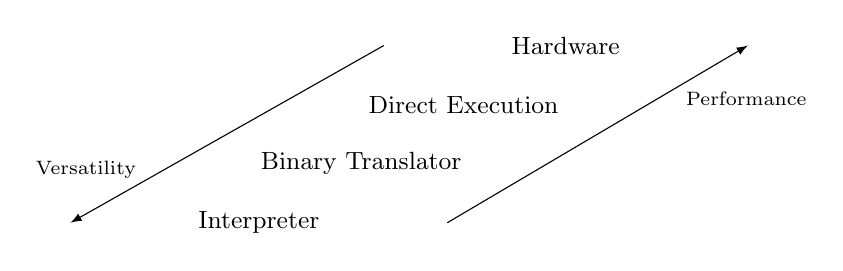
\begin{tikzpicture}[>=latex,
                    node distance=0.25cm, font=\small,
                    align=left,
                    start chain=going {at=(\tikzchainprevious),shift=(30:1.5)}]
\node[on chain] (n1) {Interpreter};
\node[on chain] {Binary Translator};
\node[on chain] {Direct Execution};
\node[on chain] (n5) {Hardware};
\coordinate[right=1.5cm of n1] (a1);
\coordinate[right=1.5cm of n5] (a5);
\coordinate[left=1.5cm of n1] (b1);
\coordinate[left=1.5cm of n5] (b5);
\pause\draw[->] (a1) -- (a5) node[inner xsep=3pt, pos=0.7, right=0.25cm] {\scriptsize Performance};
\pause\draw[->] (b5) -- (b1) node[inner xsep=3pt, pos=0.7, left=0.25cm] {\scriptsize Versatility};
\end{tikzpicture}
\end{frame}

\begin{frame}{Gear Shifting}
\centering
\inputpicture{gearbox}
\end{frame}

\begin{frame}{Dynamic Mode Switch}
\begin{itemize}
\item[$+$] Optimal usage of the best aspects of each approach.
\item[$-$] Several simulators are actually need to be developed.
\end{itemize}
\end{frame}

\section{Conclusions}

\begin{frame}{Conclusions}
\begin{itemize}
\item{<<Naive>> direct execution.}
\item Preliminary scanning.
\item Stubs and patches.
\item Hardware support for direct execution.
\item{<<Gear shiftin>> for simulation modes.}
\end{itemize}
\end{frame}

\begin{frame}[allowframebreaks]{Bibliography}
\begin{thebibliography}{99}
\bibitem{} \textit{Kevin P. Lawton}. Plex86: An 180x86 Virtual Machine.
\bibitem{} Pin - A Binary Instrumentation Tool - Papers.
  \url{https://software.intel.com/en-us/articles/pin-a-binary-instrumentation-tool-papers}
\bibitem{} \textit{Heidi Pan, Krste Asanovíc, Robert Cohn and Chi-Keung Luk}.
  Controlling Program Execution through Binary Instrumentation.
\bibitem{} \textit{F. Leung, G. Neiger, D. Rodgers, A. Santoni, R. Uhlig}.
  Intel Virtualization Technology: Hardware Support for Efficient Processor
  Virtualization.
\bibitem{} \textit{E.~Bugnion, S.~Devine, M.~Rosenblum, J.~Sugerman, E.~Wang}.
  Bringing Virtualization to the x86 Architecture with the Original VMware
  Workstation
\end{thebibliography}
\end{frame}

\begin{frame}{On the Next Lecture:}
Full-platform simulation:
\begin{itemize}
\item Timer Simulation.
\item Discrete-Event Simulation.
\item Multi-core Systems.
\item Co-Simulation.
\end{itemize}
\end{frame}

\finalslide

\end{document}
